\chapter{Introduction to Chemical Reaction Networks}\label{chap:ch1}

In this first chapter we'll start with the concepts that apply to the broader range of \text{natural sciences}.

The following picture, that's also been shown by my Professor in his presentation of this topic \parencite{Lorand2024} might be a good introduction:

\begin{figure}[H]
	\centering
	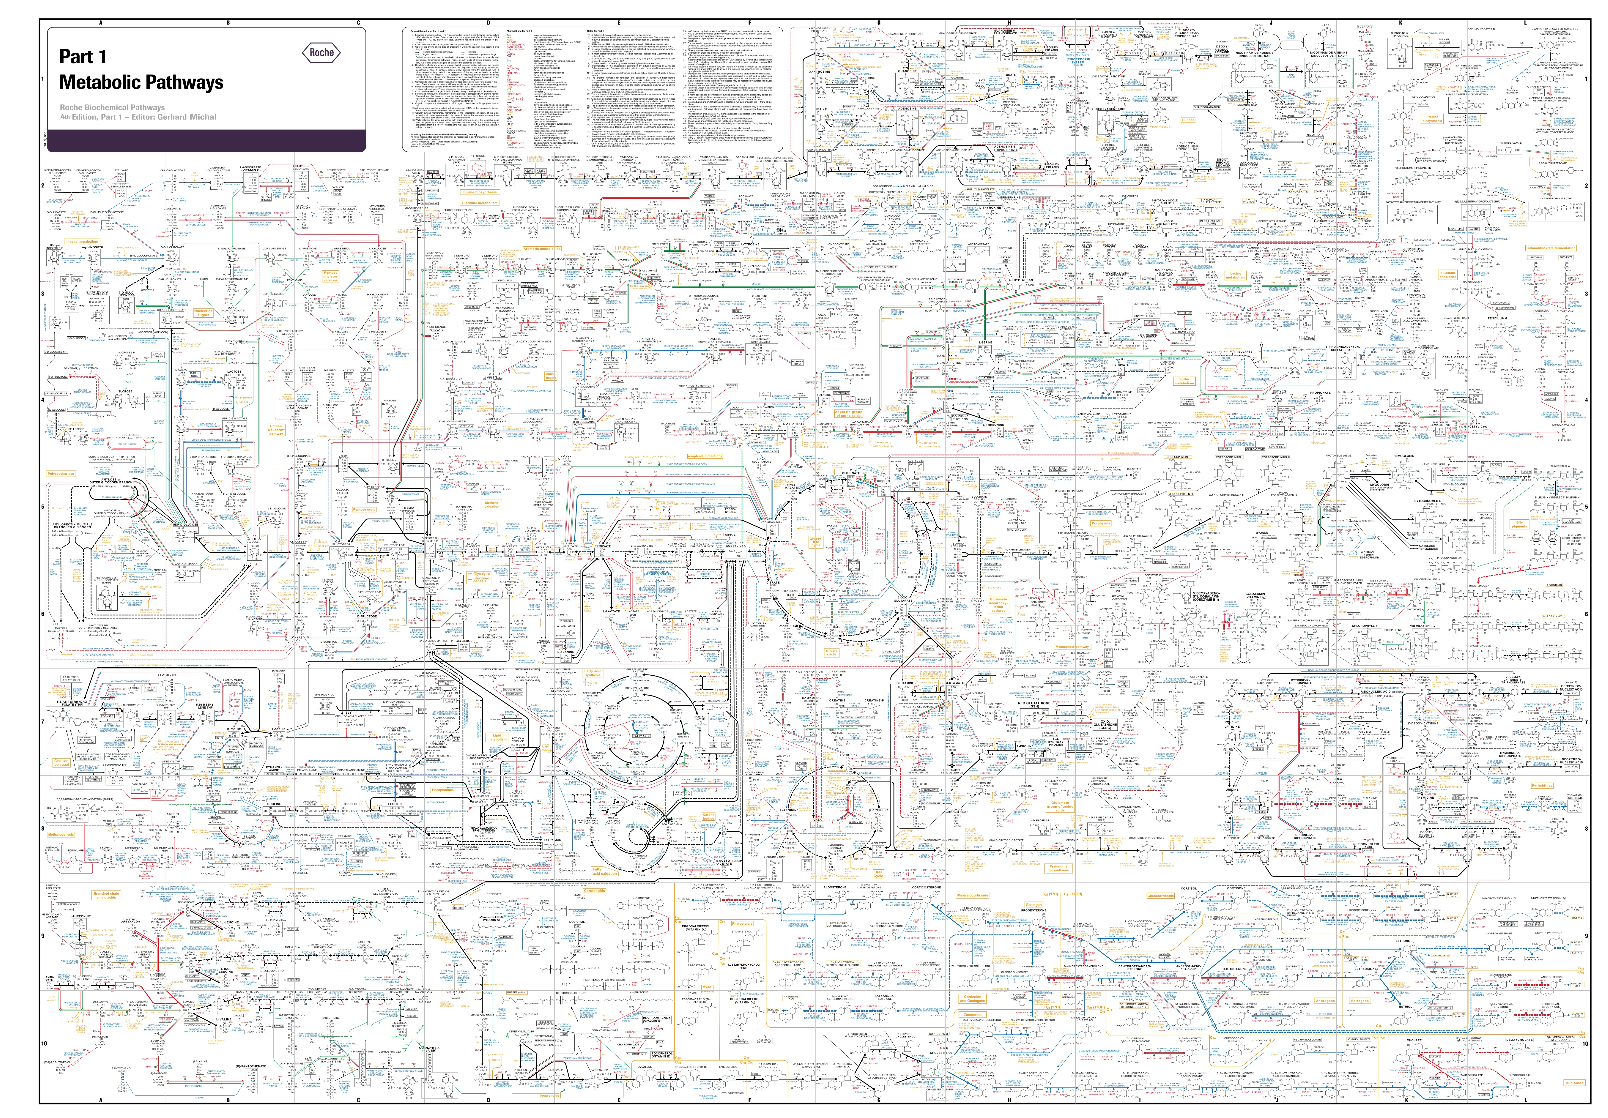
\includegraphics[width=\textwidth]{chem-pics/metabolic-pathways.png}	
	\caption{The Metabolic Pathways poster by Dr. Gerhard Michal from Roche Biochemical \cite{RouchePathways}}
	\label{fig:metabolic-pathways}
\end{figure}

We'll introduce and mathematically define Chemical Reaction Networks (CRN) consisting of:

the set $S = \left\{ X_1, \dots, X_n \right\}, \left| S \right| = n$ of chemical species,

and $r$ reactions of the form:
\begin{equation}\label{mass-action_network}
	\alpha_{1j} X_1 + \dots + \alpha_{n j} X_n \xrightarrow{k_j} \beta_{1j} X_1 + \dots + \beta_{n j}, \forall j = \overline{1,r}.	
\end{equation}

Where $\alpha_{ij}$ is the coefficient of stoichiometry of the reactant $X_i$ in reaction $j$.

The same goes for $\beta_{ij}$, but for the \textbf{produced} $X_i$ in reaction $j$. These are also called the \textbf{stoichiometries} of each reactant / product.

$k_j$ are the reactions' rate constants.

We denote the species' concentrations with $[X_1], \dots, [X_n]$.

We could shorthand both of them in their vector form:
\begin{gather*}
	x \in \mathbb{R}^n_{> 0},  k \in \mathbb{R}^r_{\geq 0} \\
	x =
	\begin{pmatrix}
		x_1 \\
		\vdots \\
		x_n 	
	\end{pmatrix}, \quad k =
	\begin{pmatrix*}
		k_1  \\
		\vdots \\
		k_r	
	\end{pmatrix*}
\end{gather*}
Now we may define the mass-action \textbf{reaction rate} of this particular reaction, which depends on the rate constant, the concentrations of reacting species and their molecularities. Part of these  presentations / definitions are taken from: \cite{Derbez2015,Lorand2024}, while part I've tried to generally define myself.
\begin{definition}
	\textbf{Reaction Rate}:	
	\begin{align}\label{reaction_rate}
		v : \mathbb{R}^r_{\geq 0}  &\bigtimes \mathbb{R}^n_{> 0} \rightarrow \mathbb{R}_{\geq 0}  \nonumber \\
		v(k,x) &= k_j [X_1]^{\alpha_{1j}} \dots [X_n]^{\alpha_{nj}} \\
		&= k_j x_1^{\alpha_{1j}} \dots x_n^{\alpha_{nj}} \nonumber
	\end{align}
\end{definition}

The way we use such a model for representing chemical reactions is with the premise that the concentrations of the species are not affected by their spatial distribution, so no funky spatial gradients and partial differential equations. Implying the "room" they have is considered necessary, the only factor in the reactions' rate being their "active mass", meaning their concentration or activity.

Otherwise, way more complex models would be used. Ones that take into account things like intermolecular interactions, the mixing process of the solution etc.

A pretty common example that you might've seen in 6th grade would be:
\[
	2H_2 + O_2 \xrightarrow{k} 2H_2O
\]
Where its reaction vector is:
\[
	\bordermatrix{\cr \cr
		H_2 & -2 \cr
		O_2 & -1 \cr
		H_2O & 2 \cr
	}
\]
with reaction rate $v(k,x) = k[H_2]^2[O_2]$. Or, by using the vector $x=(x_1, x_2, x_3, x_4)$: $v(x) = k x_1^2 x_2$.
So the reaction's dynamical system (defined more in detail in \ref{ch:dynamical_systems}) is:
\begin{align}\label{1st_example_dyn_system}
	\frac{d}{dt}
	\begin{pmatrix*}
		x_1 \\
		x_2 \\
		x_3
	\end{pmatrix*} =
	\begin{pmatrix}
		-2 \\
		-1 \\
		2
	\end{pmatrix}
	v(k,x)
\end{align}
But if we have multiple such reactions we need to use their:
\begin{definition}
	\textbf{Stoichiometric matrices.}
	\begin{align*}
		\Gamma_L, \Gamma_R &\in \mathcal{M}_{n \bigtimes r}(\mathbb{N}) \\
		(\Gamma_L)_{ij} &= \alpha_{ij} \text{ from \ref{mass-action_network}} \\
		(\Gamma_R)_{ij} &= \beta{ij} \text{ from \ref{mass-action_network}} \\
		\Gamma &\in \mathcal{M}_{n \bigtimes r}(\mathbb{Z}) \\
		\Gamma &= \Gamma_R - \Gamma_L
	\end{align*}
	$\Gamma_L$ the \textbf{left} stoichiometric matrix, \\
	$\Gamma_R$ the \textbf{right} stoichiometric matrix, and \\
	$\Gamma$ : the \textbf{full} stoichiometric matrix.
\end{definition}
So constructing their equivalent of \ref{1st_example_dyn_system}:
\begin{align}\label{crn_system_matrix_form}
	\frac{d}{dt}
	\begin{pmatrix*}
		x_1 \\
		\vdots \\
		x_n
	\end{pmatrix*} = \Gamma
	\begin{pmatrix*}
		v_1(k,x)	 \\
		\vdots \\
		v_r(k,x)
	\end{pmatrix*}
	\text{ or, even more shorthand:  }
	\frac{dx}{dt} = \Gamma v(k,x).
\end{align}
Where
\begin{definition}\label{flux_vector}
	\textbf{Flux Vector.}
	\begin{align}
		v : \mathbb{R}^r_{\geq 0}  \bigtimes &\mathbb{R}^n_{> 0} \rightarrow \mathbb{R}^r_{\geq 0}  \nonumber \\
		(v(x,k))_{i} &= v_i(k_i, x)
	\end{align}
	is a column vector of all reaction rates for the reactions. For reasons later discussed in \ref{convex_paramteres}, we will call it the \textbf{flux vector.}
\end{definition}

\newpage
\textbf{Example}\label{bigger_network_example1} 1:
One such bigger network would be the following \textbf{open network}.
\begin{align*}
	A + C \xrightarrow{k_{1}} 2A \\
	B + C \xrightarrow{k_{2}} 2B  \\
	A \xrightarrow{k_{3}} 0 \\
	B \xrightarrow{k_{4}} 0 \\
	0 \xrightarrow{k_{5}} C
\end{align*}
To indicate interaction with the "outside" world (kind of like an interface to the outside world).
Here: 	

$C$ is like a "resource" molecule.

$A$, $B$ \textbf{autocatalyze} themselves with $C$, so they produce themselves as they go, until they use $C$ up and one of them ends up on top, depending on their initial concentrations, so this system would also be \textbf{bistable}.

This system would look like:
\begin{align*}
	\Gamma_L =
	\begin{pmatrix}
		1 & 0 & 1 & 0 & 0 \\
		0 & 1 & 0 & 1 & 0 \\
		1 & 1 & 0 & 0 & 0
	\end{pmatrix}
	, \quad
	\Gamma_R =
	\begin{pmatrix}
		2 & 0 & 0 & 0 & 0 \\
		0 & 2 & 0 & 0 & 0 \\
		0 & 0 & 0 & 0 & 1
	\end{pmatrix}
\end{align*}
\begin{equation*}
 \Gamma =
 \begin{pmatrix*}
		1 & 0 & -1 & 0 & 0 \\
		0 & 1 & 0 & -1 & 0 \\
		-1 & -1 & 0 & 0 & 1
 \end{pmatrix*}
\end{equation*}
Whereas, the reaction rate:
\[
	v(k,x) =
	\begin{pmatrix*}
		v_{1}(k,x)	 \\
		v_{2}(k,x)	 \\
		v_{3}(k,x)	 \\
		v_{4}(k,x)	 \\
		v_{5}(k,x)
	\end{pmatrix*} =
	\begin{pmatrix}
		k_1 x_1 x_3 \\
		k_2 x_2 x_3 \\
		k_3 x_1 \\
		k_4 x_2 \\
		k_5
	\end{pmatrix}
\]
And so its dynamical system in matrix form is:
\begin{align*}
	\frac{dx}{dt} &= \Gamma v(k,x) \\
	\frac{d}{dt}
	\begin{pmatrix*}
		x_1	\\
		x_2	\\
		x_3	
	\end{pmatrix*} &=
	\begin{pmatrix*}
		1 & 0 & -1 & 0 & 0 \\
		0 & 1 & 0 & -1 & 0 \\
		-1 & -1 & 0 & 0 & 1
 \end{pmatrix*}
	\begin{pmatrix}
		k_1 x_1 x_3 \\
		k_2 x_2 x_3 \\
		k_3 x_1 \\
		k_4 x_2 \\
		k_5
	\end{pmatrix}
\end{align*}
As you can see this is the same as \ref{1st_example_dyn_system}, I just didn't use the notation " $\Gamma$ " then. This results in:
\[
	\begin{cases*}
		\dot{x}_1 = k_1 x_1 x_3 - k_3x_1  \\
		\dot{x}_2 = k_2 x_2 x_3 - k_4 x_2  \\
		\dot{x}_3 = -k_1 x_1 x_3 - k_2 x_2 x_3 + k_5 \\
	\end{cases*}
\]

\textbf{Interaction graphs} (first encountered this term in \cite{Derbez2015}): Every chemical reaction network has its corresponding interaction graph, formed of the following basic structure.

Two intersecting arrows mean a sum of the reacting / produced species.

So for reactions of the form
\begin{align*}
	B + A \xrightarrow{k_{1}} D + C
\end{align*}
Their interaction graph would be:
\usetikzlibrary{arrows.meta, positioning}

\begin{center}
	\begin{tikzpicture}[>=Stealth, node distance=2cm]
		\centering
		\node (B) {B};
		\node[below=1.2cm of B] (A) {A};
		\node[right=3cm of A] (C) {C};
		\node[right=3cm of B] (D) {D};

		\draw[->, bend left=45] (A) to (C);
		\draw[->, bend right=45] (B) to (D);
	\end{tikzpicture}
\end{center}

We'll use these kinds of figures in later chapters, when talking about more specific CRN's.
But one thing that's certain is these CRN's can also be modeled by the concept discussed in this next chapter.